\begin{figure}[!htb]
    \centering
    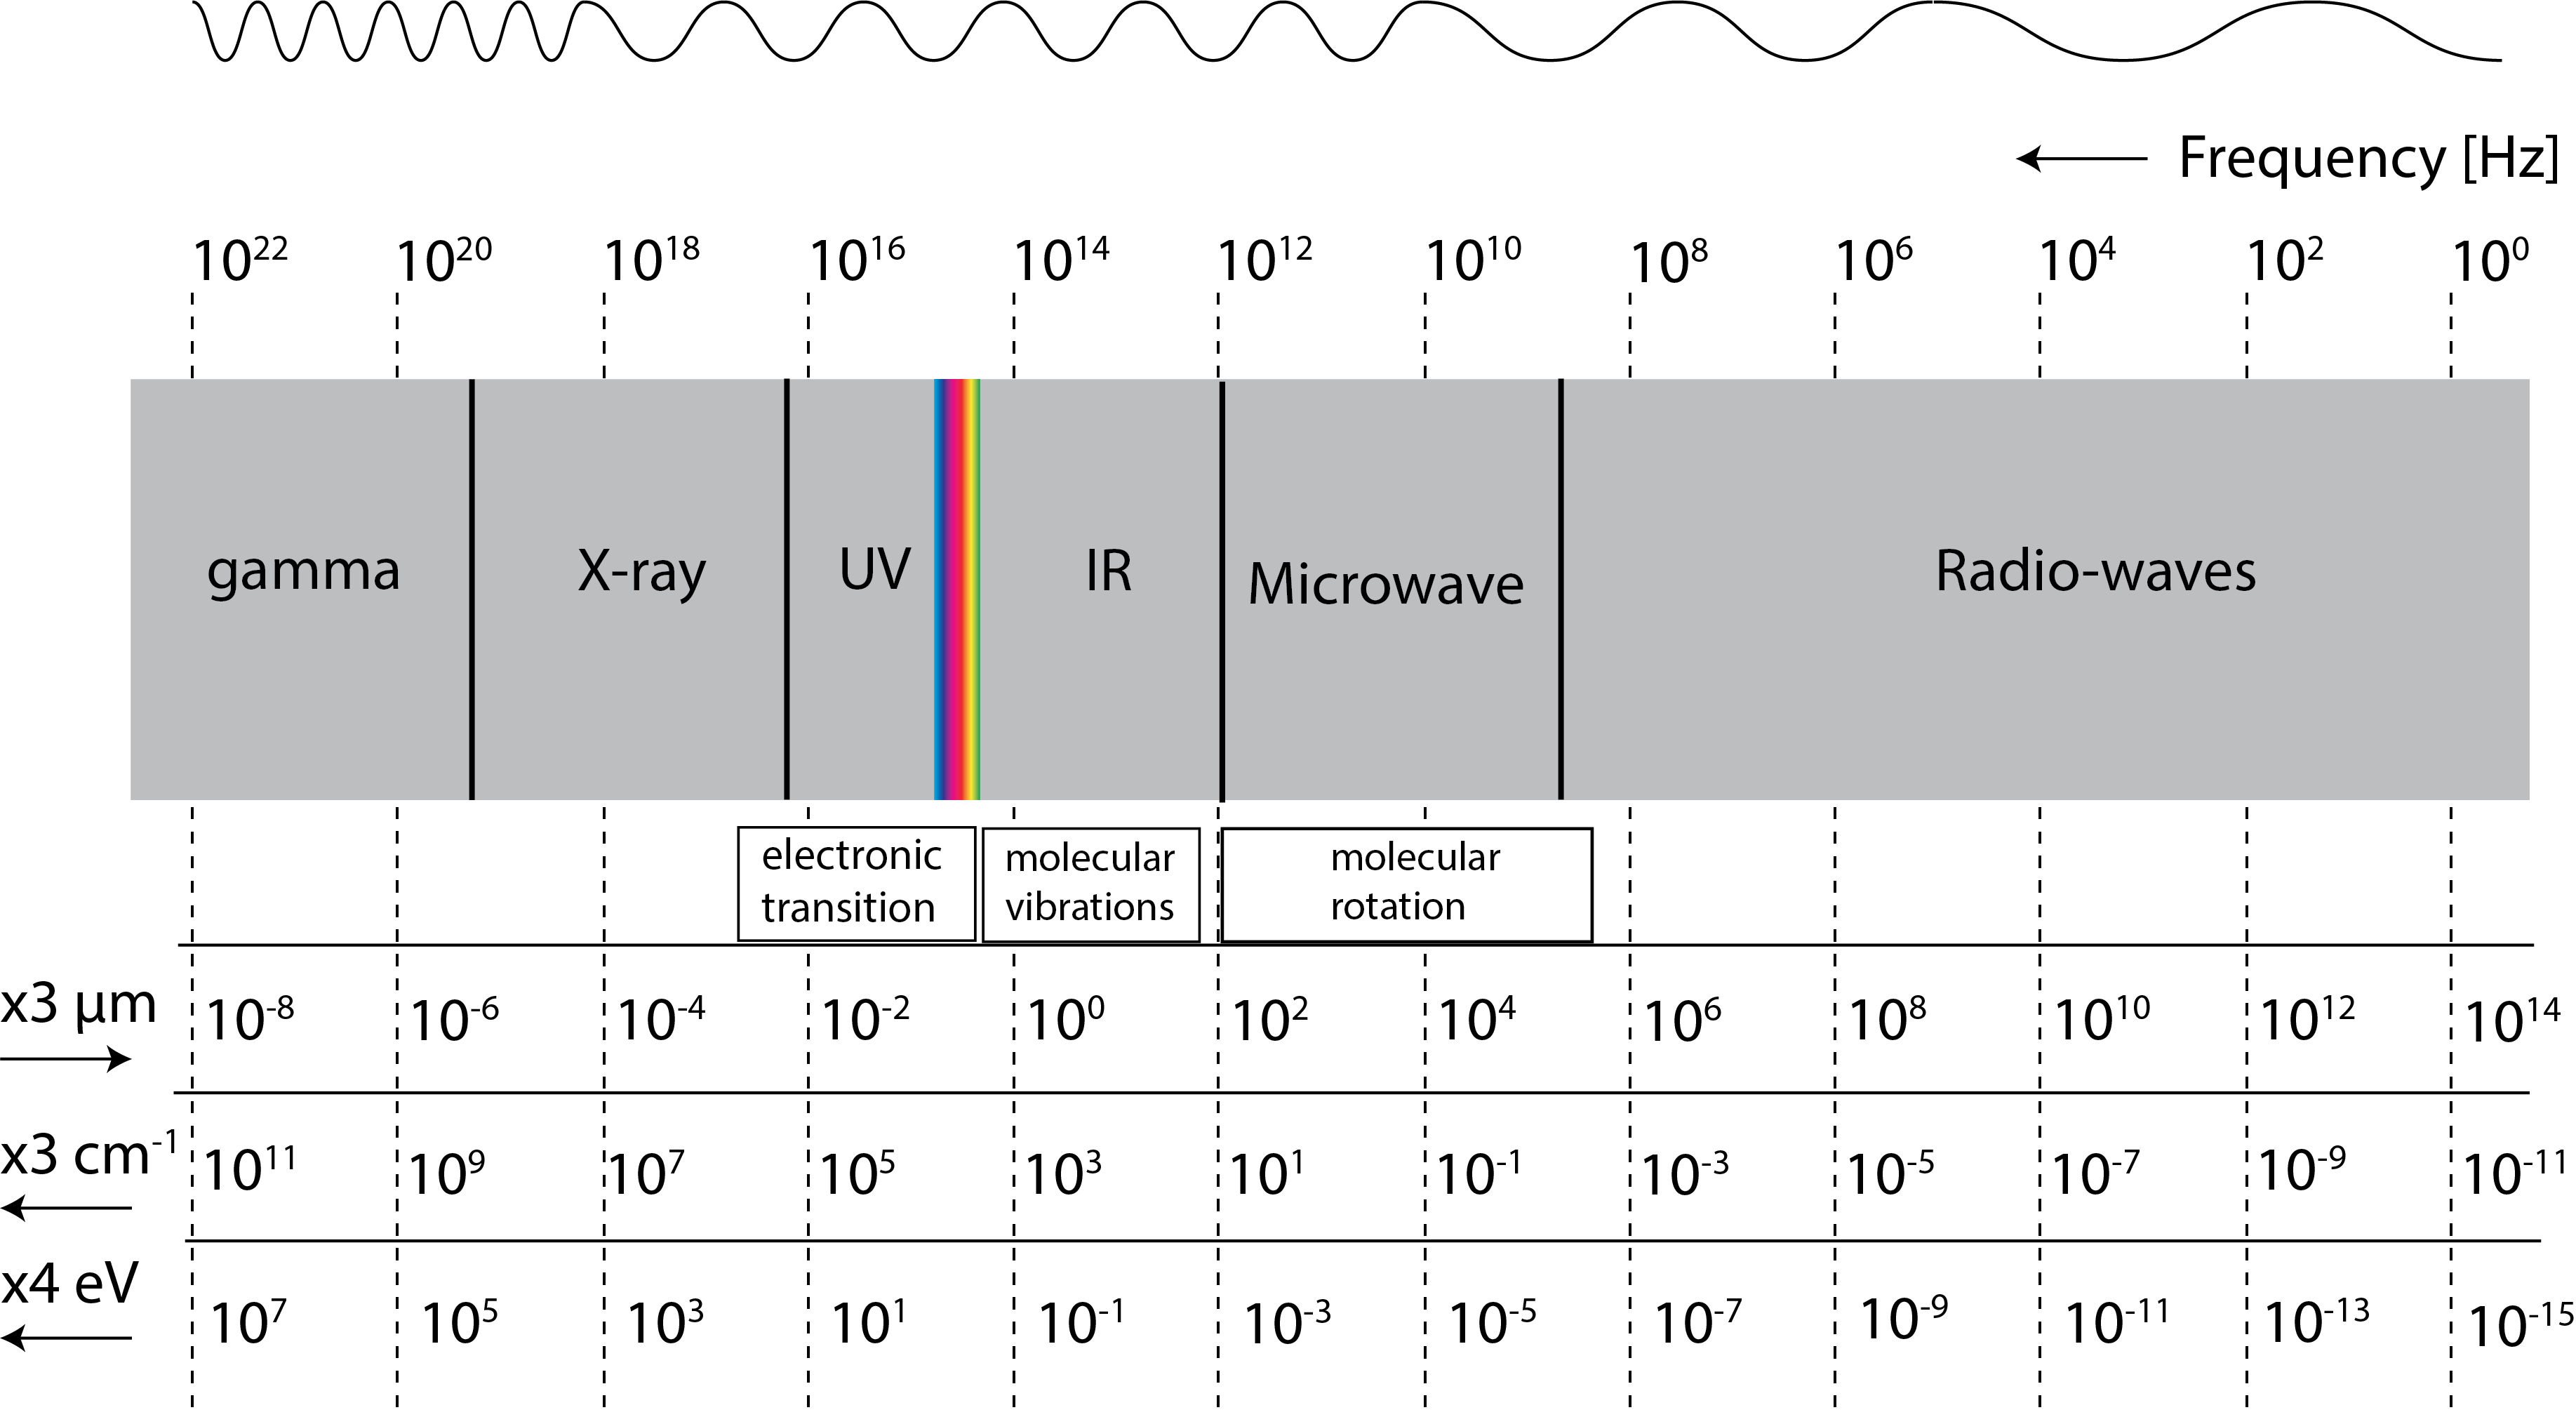
\includegraphics[width=0.9\textwidth]{figures/intro/EM_spectrum_1.png}
    \caption{Schematic diagram of the electromagnetic spectrum, the rainbow-coloured inset shows the visible spectrum. The vertical dashed line indicates a corresponding comparison to the different unit systems as labeled on the left, and \qt{x3} and \qt{x4} indicate that the scale value is multiplied by factors 3 and 4, respectively.}
    \label{fig:EM_spectrum}
\end{figure}

\begin{table}[!htb]
    \centering
    \caption{Dominant types of molecular transitions in each region of the electromagnetic spectrum}
    \begin{tabular}{lccc}
        \toprule
        \multicolumn{2}{c}{\textbf{Region of Spectrum}} & \textbf{Energy [cm$^{-1}$]} & \textbf{Molecular transitions} \\\midrule
        \multicolumn{2}{c}{\emph{Ultraviolet (UV)}} && \multirow{4}*{Electronic}\\
        & far & $10^6 - 50,000$ & \\
        & near & $50,000 - 26,300$ & \\
        \addlinespace
        \multicolumn{2}{c}{\emph{Visible (Vis)}} & $26,300 - 12,800$ & \\
        \midrule\addlinespace
        \multicolumn{2}{c}{\emph{Infrared (IR)}} && \multirow{4}*{Vibrational} \\
        & near & $12,800 - 4000$ & \\
        & mid  & $4000 - 200$ & \\
        & far  & $200 - 10$ & \\
        \midrule\addlinespace
        \multicolumn{2}{c}{\emph{Microwave (THz)}} & $10 - 0.01$ & Rotational \\
        \bottomrule\hline\\
    \end{tabular}
    \label{tab:electromagnetic_spectrum}
\end{table}
